% Primarily this section should be about scientific methods and theories you need to evaluate/compare/invent to solve your problems from 1.3.
% In some cases it may be ok to describe different technologies, but the purpose is to describe something and then draw a conclusion from that.
% Example, if you decide to discuss different databases, it may be for the purpose of selecting the best type for your implementation later on (based on for example data representation, scalability, speed, etc.).
% Optimally the problems in 1.3 are not solved by anyone else yet, in which case this section needs to describe how to solve them (new algorithms, mathematical approaches, etc.).
 
% This section can have a lot of subsections (3.1, 3.2, 3.3, etc).

The values of a program needs to be temporary stored some were on the computer were it can easily be access while running the program.
The two ways the computer can do this is to either store it in a register or in the memory.
Registers are very limited in space and are very volatile thus it is good for storing values that are needed often in a short amount of time.
Memory is slower but has a lot more space and is thus much more useful for storing values that will be needed in a while.
The compiler will compile the program to store the different variables and values in the registers and memory in a structured way so it is easily managed.

There is no real structure for the registers except that certain registers have a specific purpose, which can be the program counter for example.
A program counter is a register that keeps track of which machine code instruction the program is currently at.
There are other important registers like the stack pointer register and more.

On the other hand the memory is structure like a stack that consist of stack frames/call frames, the stack is usually called the \emph{call stack}.
A stack is a data structure that consist of a number of elements that are stacked on top of each other and the only two operations available for a stack is push and pop.
The push operations adds a new element on top of the stack and the pop operation removes the top element of the stack.
Other key characteristics are that it is only the top element that can be access thus to reach the lower elements all the above elements needs to be poped.


\begin{figure}[h]
    \centering
    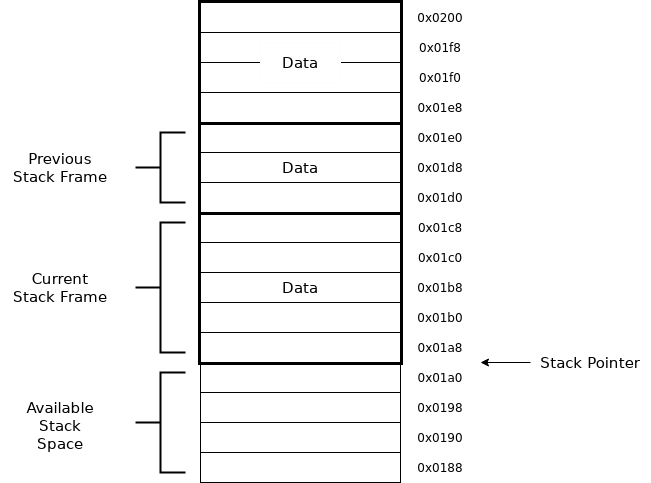
\includegraphics[width=1.0\textwidth]{call-stack.png}
    \label{fig:callstack}
\end{figure}


\subsubsection{Call Stack}
% \import{theory/}{dwarf.tex}


\subsubsection{Stack Frame/Call Frame}
% \import{theory/}{dwarf.tex}

